%!TEX root = ../Thesis.tex
%!TEX program = xelatex
\documentclass[../Thesis]{subfiles}


% 本文
\begin{document}
\chapter{手法}
\section{概要}
  提案手法の概要図を\fref{img01}に示す.提案手法では、ドローン空撮映像を切り取ったフレーム画像を入力画像とし、前処理を行う。その後、災害領域と不要領域を検出し、災害領域検出結果より不要領域検出結果を除去した斜面崩壊と浸水領域の検出結果を最終出力結果とする。

  \begin{figure}[h]
		\centering
		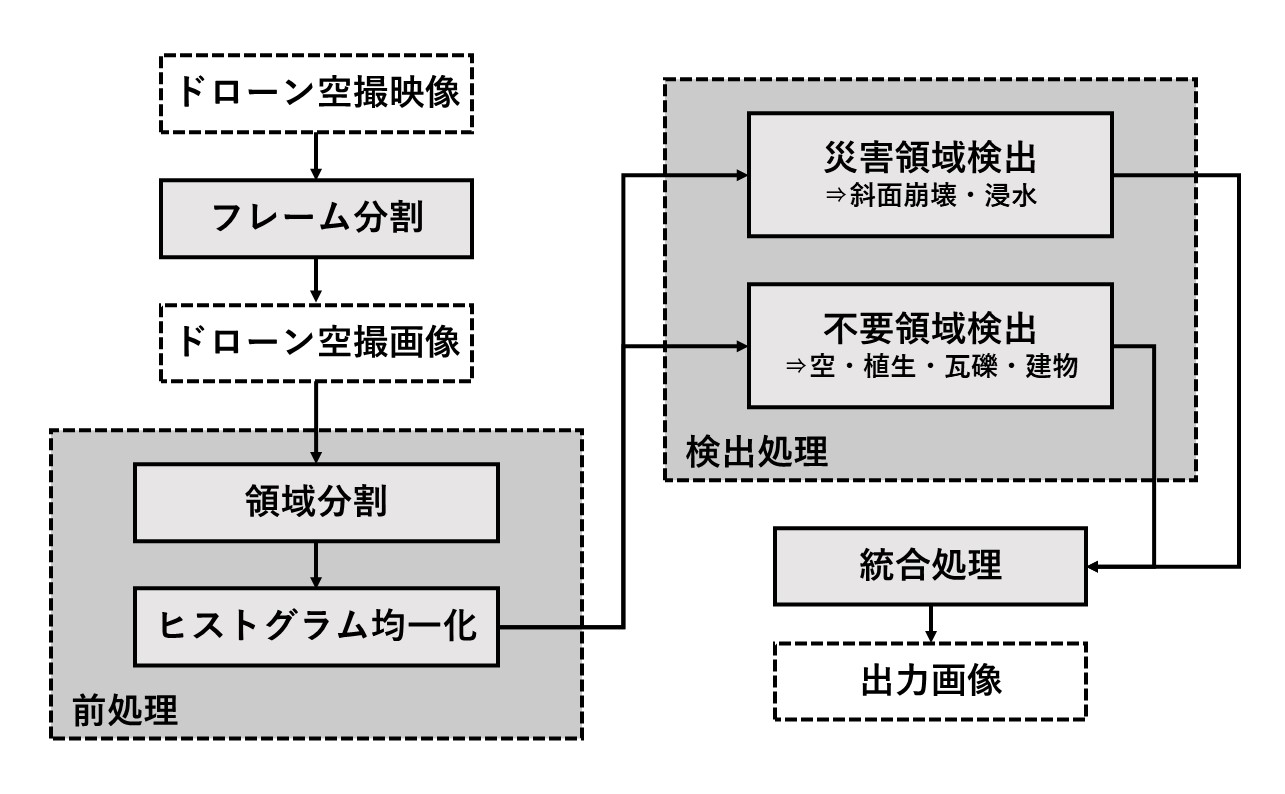
\includegraphics[width=8cm]{img/howto.jpg}
		\caption{提案手法概要図}
		\label{img01}
  \end{figure}
  

\section{領域分割}
  斜面崩壊・浸水領域を画素単位で検出することは難しいため、近傍画素との関係性を考慮した上で領域単位で判別を行う。本研究ではMean-Shift法を用いた領域分割を行う。Mean-Shift法はカーネル密度推定によるクラスタリング手法の一つで画像の領域分割、動画像における対象物体追跡に用いられる。また、領域分割の代表的な手法であるk-means法に比べ、クラスタ数を事前に決める必要が無い。d次元空間中のN個の点群$x_i$を標本として得られるような確率密度関数$f(x)$を考え、その標本点から確率密度関数$f(x)$の極大点を探索する手法である。
  次に、Mean-Shift法にてカラー画像の領域分割を行う手順について説明する。

  \begin{enumerate}
    \item カラー画像中の各画素の位置を二次元座標$x_i$、その画素値を三次元チャンネル$v_i=(R_i,G_i,B_i)$とし、画素位置と画素値を結合した5次元空間内の点$z_i=(x_i,v_i)$を考える。距離と色相が近い画素が5次元空間内でクラスタを成しているとし、各画素をMean-Shift法でクラスタリングする。
    \item 画素位置、画素値のバンド幅をそれぞれ$h_s,h_r$とする。すべての$z_i$にMean-Shift法を適用し、収束位置$z^c=(x^c,v^c)$を計算する。
    \item $x_i$の画素値を収束位置の画素の値$v_i=(R_i,G_i,B_i)$に置き換えることによって領域分割ができる。
  \end{enumerate}
  
  なお、$x^s,x^r$をそれぞれ5次元ベクトルの空間に対応するものとし、カーネル密度推定を以下{式x}のように定義することでMean-Shift法は以下のように計算される。

  \begin{equation}
    f(x) = \frac{c}{Nh_s^2h_r^3} \sum_{i=1}^N k (|\frac{x^s-x_i^s}{h_s}|^2) k (|\frac{x^r-x_i^r}{h_r}|^2)
  \end{equation}

  \begin{equation}
    y_{j+1}^s = \frac{\sum_{i=1}^N g_i^sx_i^s}{\sum_{i=1}^N g_i^s}, y_{j+1}^r = \frac{\sum_{i=1}^N g_i^rx_i^r}{\sum_{i=1}^N g_i^s}
  \end{equation}

  ただし、
  \begin{equation}
    g_i^s = k' (|\frac{y_j^s-x_i^s}{h_s}|^2) k (|\frac{y_i^r-x_i^r}{h_r}|^2), g_i^r = k (|\frac{y_j^s-x_i^s}{h_s}|^2) k' (|\frac{y_i^r-x_i^r}{h_r}|^2)
  \end{equation}
  である。
  
  なお、本研究ではMean-Shift法の特徴量空間に距離を表す画素位置(x,y)、色相を表す画素値(R,G,B)を用いるので5次元空間での処理となり、距離、色相の近しい画素群が一つの領域となる。領域分割の適用例を\fref{img02}に示す。

  \begin{figure}[h]
		\centering
		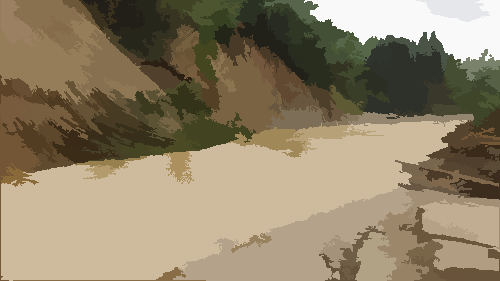
\includegraphics[width=8cm]{img/ex_meanshift.jpg}
		\caption{領域分割適用例}
		\label{img02}
  \end{figure}


\section{ヒストグラム均一化}
  空撮画像は撮影時の天候や時刻、季節によって色相や輝度に偏りが生じる。本研究では色相や輝度、色情報を用いた指標によって判別処理を行うので偏りによって検出結果に影響が生じる可能性があるのでCLAHEのアルゴリズムによってヒストグラムを均一化する。\cite{art05}。CLAHEのアルゴリズムとは画像をタイルと呼ばれる小領域に分割し、タイル毎にヒストグラム均一化を行う手法である。ただし、タイル毎に均一化を行うとノイズが強調されるため、ビンの出現頻度が特定の上限値以上となった場合、その画素をその他のビンに均等に配分した後ヒストグラムの均一化を行うことによってノイズの強調を抑える。よって、本研究ではCLAHEのアルゴリズムによってノイズの強調を抑えつつヒストグラムの均一化を行う。ヒストグラム均一化の適用例を\fref{img03}に示す。

	\begin{figure}[h]
		\centering
		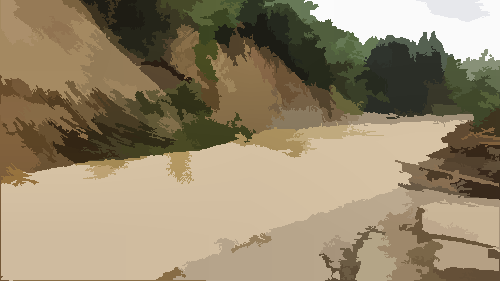
\includegraphics[width=8cm]{img/ex_equalization.jpg}
		\caption{ヒストグラム均一化適用例}
		\label{img03}
  \end{figure}


\section{災害領域検出}
% \section{斜面崩壊・浸水領域検出}
  斜面崩壊・浸水領域での色情報や輝度情報等の特徴を\tref{tab01}に示す。これらの特徴を用いて各領域の検出を行う。
  
	\begin{table}[b]
		\centering
		\caption{各災害領域の特徴}
		\label{tab01}
		\begin{tabular}{c c c c c}
			\hline
			領域名 & 色相 & 彩度 & 輝度 & 均一度 \\
			\hline
			\hline
			斜面崩壊 & 赤 & 高 & 低 & -- \\
			浸水 & 赤 & 低 & 高 & 高 \\ \hline
		\end{tabular}
	\end{table}

\subsection{L*a*b*変換}
  前述の各災害領域の特徴に従って分類を行うためヒストグラム均一化を行った画像に対しL*a*b*変換を行う。L*a*b*色空間とは輝度をL*、色相と彩度を示す色度をa*,b*で表した色空間である。また、人間の視覚に近い色空間であり、色情報にて分類を行う際に有効な指標である。本研究で用いている画像は現時点ではRGB色空間にて表されているためL*a*b*色空間への変換を行う。RGB色空間からL*a*b*色空間への変換式を{}~{}に示す。なお、RGB色空間はデバイス依存色であり、これかららららから直接L*a*b*色空間に変換する式は存在しないためデバイス独立色であるXYZ色空間に変換してから処理を行う。XYZ色空間への変換は0から255までの8bit値を0から1に変換し、γ=2.2に対するガンマ補正を線形の測定値に戻す。
  
  なお、EはR,G,Bのいずれかを表し、ダッシュ付きはガンマ補正された値を示す。
  
  \begin{equation}
    L* = 116 \times f(\frac{Y}{Y_n}) - 16
    a* = 500 \times f(\frac{X}{X_n}) - f(\frac{Y}{Y_n}))
    b* = 200 \times f(\frac{Y}{Y_n}) - f(\frac{Z}{Z_n}))
  \end{equation}
  \begin{equation}
    X = 0.4124R+0.3576G+0.1805R
    Y = 0.2126R+0.7152G+0.0722R
    Z = 0.0193R+0.1192G+0.9505R
  \end{equation}

  ただし、
  \begin{equation}
    E' = E'_{8bit}/255.0
    E = E'/12.92 E'<=0.04045
    ((E'+0.055)/1.055^2.4) E'>0.04045
  \end{equation}
  
  \begin{equation}
    f(t) = 
    t^{\frac{1}{3}} t>(\frac{6}{29}^3) \\
    \frac{1}{3}(\frac{29}{6})^2t+\frac{4}{29} t<=(\frac{6}{29}^3)
  \end{equation}
  とする。

  また、RGB色空間画像に対しL*a*b*変換を適用した例を\fref{}に示す。????いらんかも




\subsection{HSV変換}
  前項同様ヒストグラム均一化を行った画像に対しHSV色空間変換を行う。HSV色空間とは色相(Hue),彩度(Saturation),明度(Value)の三成分からなる色空間でありこれらの成分を用いて分類を行う際に有効な指標である。よって、RGB色空間で表されたヒストグラム均一化画像に対しHSV色空間変換を行う。RGB色空間からHSV色空間への変換式を{}~{}に示す。なお、R,G,Bは0から1の範囲に正規化してあるとする。

  \begin{equation}
    E = E / 255.0
    Max = Max(R,G,B)
    Min = Min(R,G,B)
    H = \frac{G-B}{Max-Min} \times 60 Max = R
    H = \frac{B-R}{Max-Min} \times 60 + 120 Max = G
    H = \frac{R-G}{Max-Min} \times 60 + 240 Max = B
    H = 0 Max = Min
    S = Max - Min
    V = Max
  \end{equation}

  また、RGB色空間画像に対しHSV変換を適用した例を\fref{}に示す。????いらんかも


% \subsection{テクスチャ解析}
%   前項同様xxxxx画像に対しテクスチャ解析を行う。テクスチャ解析とは画像内の領域を輝度パターンによって特徴付ける処理であり、リモートセンシングで土地被覆の分類に用いられることがある。本研究ではテクスチャの統計的特徴量を求めるために離れた2つの場所にある画素対の値から画素値の一様性、方向性、コントラストなどの表す特徴量を求める同時正規行列を用いる。
%   次に、同時正規行列の求め方について説明する。\fref{img00}に示すようなある画素iとjの画素対について相対的な距離をδ=<d,θ>とする。それぞれの画素値をL_i,L_jとし、画素値の対(L_i,L_j)が生じる出現頻度である同時正規行列H_δ(L_i,L_j)を考える。ここで、出現頻度の総数でH_δ(L_i,L_j)を正規化し確率に変換した同時正規行列をP_δ(L_i,_j)とする。デジタル画像ではd=1の場合θのとりうる値は0°,45°,90°,135°,180°,225°,270°,315°となる。図xに求め方例を示す。
%   本研究では画層の不均一度を表す指標である異質度を用いる。異質度は周辺画素との差が大きいと値が大きくなる指標であり、土砂や瓦礫等の検出に有効な指標である。異質度を求める式を{}に示す。

% 	\begin{figure}[h]
% 		\centering
% 		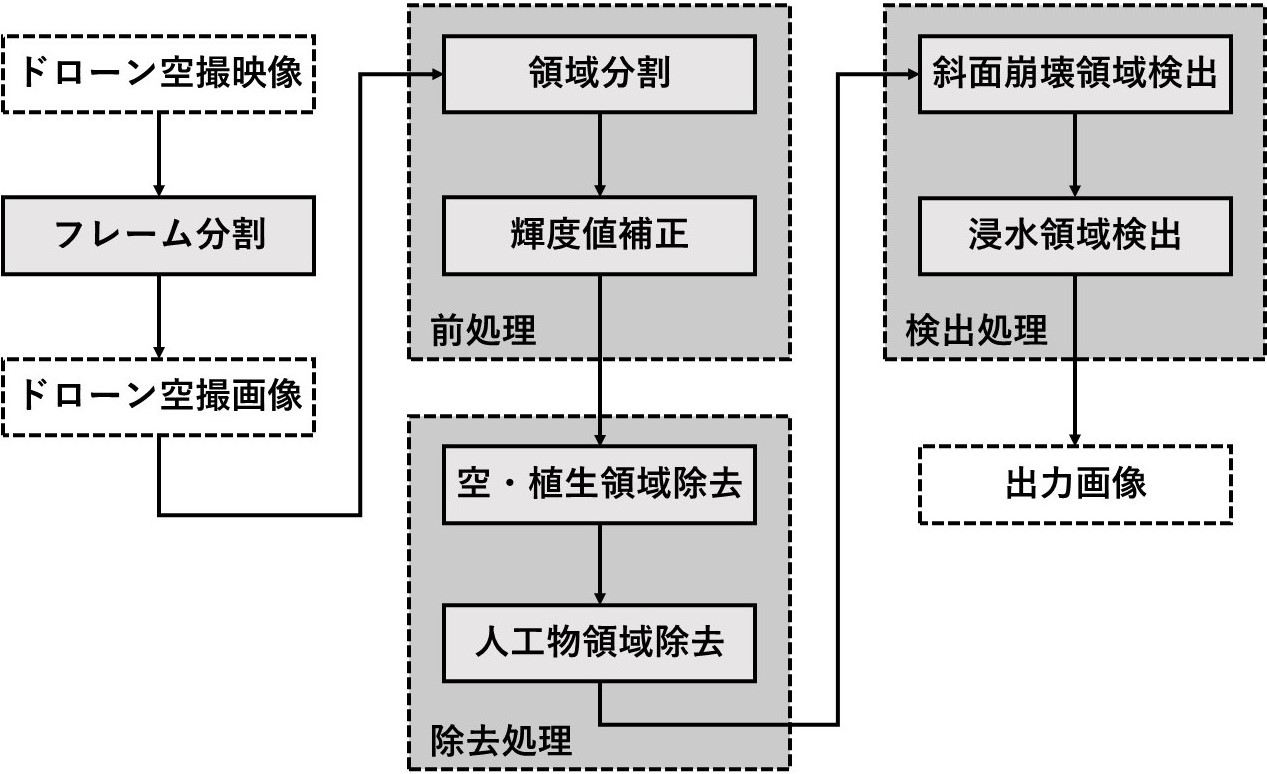
\includegraphics[width=8cm]{img/howto3.jpg}
% 		\caption{同時正規行列}
% 		\label{img00}
%   \end{figure}

%   \begin{equation}
%     dissimilitarity = \frac{1}{2}(\sum_{255}^{i=0}\sum_{255}{j=0}P_{δ1}(i,j)|i-j|+\sum_{255}^{i=0}\sum_{255}{j=0}P_{δ2}(i,j)|i-j|)
%     dissimilitarity = \sum_{255}^{i=0}\sum_{255}{j=0}P_δ(i,j)|i-j|
%   \end{equation}

\subsection{斜面崩壊領域}
  斜面崩壊領域は\tref{tab01}に示すように、輝度と色相、彩度に特徴を持つ。よって、これらの特徴を表すL*a*b*色空間のL*値とa*値、HSV色空間のS値を用いる。ヒストグラム均一化処理後の画像に対しL*a*b*色空間変換とHSV色空間変換を行い、これらの指標を用いた閾値処理により斜面崩壊領域を検出する。


\subsection{浸水領域}
  浸水領域は\tref{tab01}に示すように,色相と彩度,輝度,均一度に特徴を持つ.よって,前項同様にL*値,a*値,S値を利用することに加えて,均一度の指標としてエッジの有無を用いることで,領域が滑らかなテクスチャかの判定を行う.このとき,エッジの検出にはCanny法を利用し,領域単位でエッジ抽出率を算出する.そして,色相等の指標と領域単位でのエッジ抽出率による閾値処理によって浸水領域を検出する.


\section{不要領域検出}
  各不要領域の特徴を\tref{tab02}に示す.2.3節と同様にこれらの特徴を用いて各領域の検出を行う.
  
	\begin{table}[b]
		\centering
		\caption{各不要領域の特徴}
		\label{tab02}
		\begin{tabular}{c c c c c}
			\hline
			領域名 & 色相 & 彩度 & 輝度 & 均一度 \\
			\hline
			\hline
			空 & 青 & -- & 高 & -- \\
			植生 & 緑 & -- & -- & -- \\
			瓦礫 & -- & -- & -- & 低 \\
			建物 & -- & -- & -- & 高 \\ \hline
		\end{tabular}
	\end{table}

% \begin{table}[h]
%   \centering
%   \caption{各災害領域の特徴}
%   \label{tab01}
%   \begin{tabular}{l l l l l l}
%     領域名 & L* & a* & b* & IRR & dis \\
%     \hline
%     \hline
%     空 & 高い & - & 低い & - & - \\
%     植生 & 低い & 低い & 低い & - & - \\
%     瓦礫 & - & - & - & - & 高い \\
%     建物 & - & - & - & 高い & 低い \\
%   \end{tabular}
% \end{table}

\subsection{GSI}
  建物領域の屋根や壁は均一度が高いため、表面粒径サイズが大きいほど高い値を示すGSI(Grain Size Index)を特徴量として用いる。R、G、BをRGB色空間の各値としてGSIの算出式を式1に示す。
  
  \begin{equation}
    {\rm GSI} = \frac{R-B}{R+B+G} \nonumber \\
  \end{equation}

  本研究では、ある領域中の全画素のGSIを算出し、GSIが閾値より低い画素の方が多い場合建物領域とする。なお、領域分割後の画像に対してGSIを算出すると粒度情報が失われるため、入力画像に対して行う。
  
\subsection{エッジ抽出}
  画像中で輝度値の変化が著しい箇所をエッジという。浸水領域は表面が均一であるためエッジが少なく、瓦礫領域は表面が不均一であるためエッジが多いという特徴がある。よって、エッジを抽出し、特徴量として用いる。本研究では、ある領域中の全画素数の内、Sobelフィルタにて抽出されたエッジ強度が閾値より高い画素数の割合(エッジ抽出率)を指標の一つとして用いた閾値処理によって浸水・瓦礫領域を検出する。なお、エッジ抽出は領域分割後の画像に対して行うとエッジ情報が失われるため、入力画像に対して行う。また、3×3のSobelフィルタを\fref{img}に示す。

	\begin{figure}[h]
		\centering
		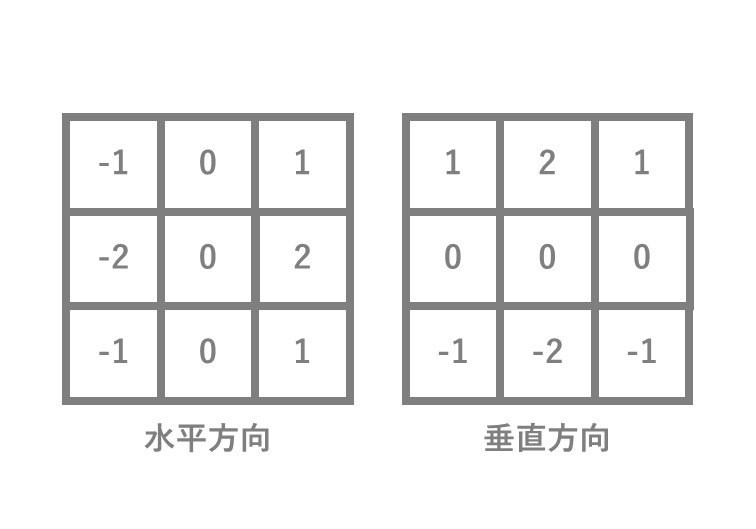
\includegraphics[width=8cm]{img/sobel.jpg}
		\caption{Sobelフィルタ(3×3)}
		\label{img03}
  \end{figure}

  \fref{img}に示したフィルタにて水平方向の微分成分d_xと垂直方向の微分成分d_yを求め、式xよりエッジ強度(S)を算出する。
  \begin{equation}
    S = \sqrt{d_x^2}{d_y^2} \\
  \end{equation}

  また、Sobelフィルタによるエッジ抽出適用例を\fref{img00}に示す。
  

\subsection{空領域}
  空領域は浸水領域同様に輝度が高く誤検出が発生する可能性がある.よって,\tref{tab02}で示した空領域の特徴から,2.3節同様にL*値とb*値を用いた閾値処理によって空領域を検出する.
  
\subsection{植生領域}
  斜面崩壊は植生を多く含む山間部の斜面にて発生し、誤検出が発生する可能性がある.よって,\tref{tab02}で示した植生領域の特徴から,a*値を用いた閾値処理によって植生領域を検出する.
	
\subseciton{瓦礫領域}
  瓦礫領域は災害領域と色相が類似しており本研究の災害領域検出手法では誤検出が発生する可能性がある。よって,瓦礫領域が多量のエッジを含むという特徴から2.3節と同様にエッジ抽出率を算出し,抽出率が高い領域を瓦礫領域とする.  

\subseciton{建物領域}
  建物領域は災害領域と色相が類似していることが多く誤検出を起こしやすいため除去する.建物領域の屋根や壁は均一度が高いためGSIを領域単位で算出し,GSIが閾値より低い画素の多い領域を建物領域とする.

\end{document}
